\documentclass[12pt]{article}
\usepackage[utf8]{inputenc}
\usepackage{graphicx}
\usepackage{amsmath}
\usepackage{amsfonts}

\title{DD Lab 4 Assignment}
\author{Sai Kartik \\2020A3PS0435P}

\begin{document}
\maketitle
\section*{7 Segment display}
\begin{center}
    \begin{figure}[ht]
        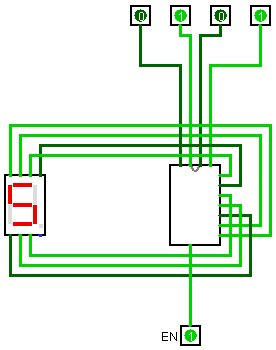
\includegraphics[scale=0.5]{sevenseg.png}
        \caption{The seven segment display}
    \end{figure}
\end{center}
\newpage
\section*{Decoder circuit}
\begin{center}
    \begin{figure}[ht]
        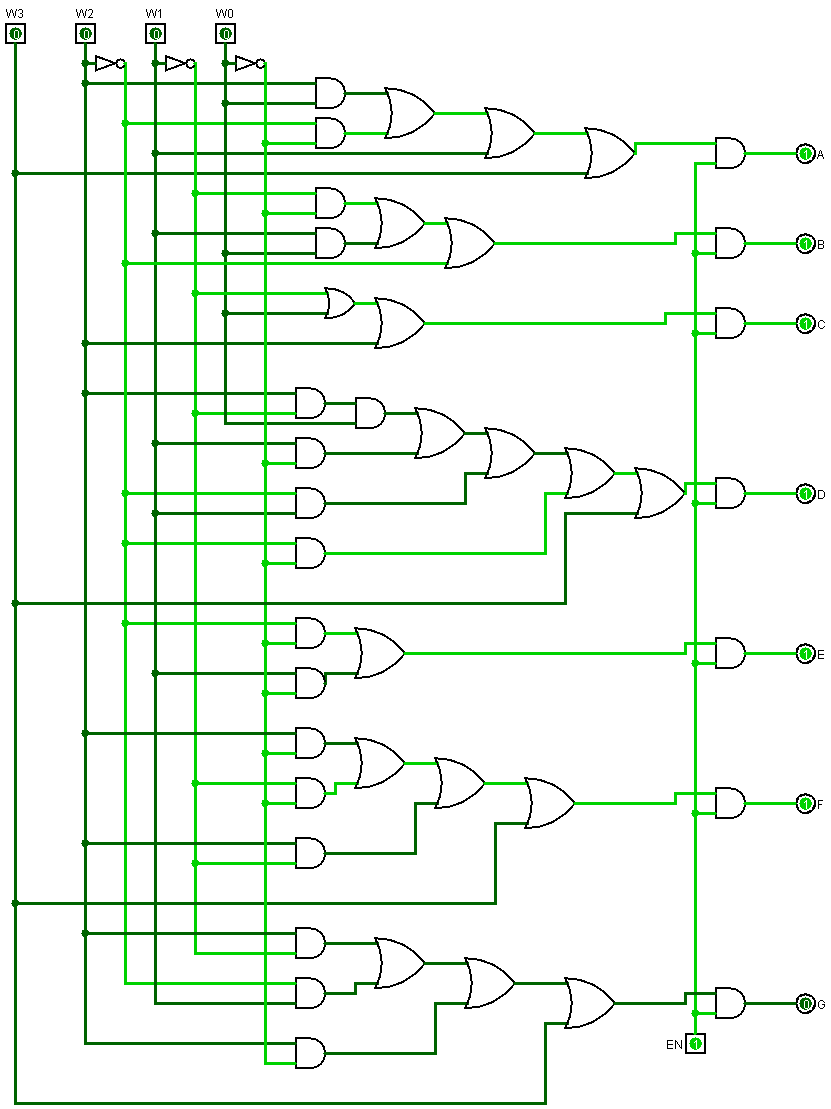
\includegraphics[scale=0.3]{decoder.png}
    \end{figure}
\end{center}
\newpage
\section*{Truth Table used to design the decoder}
The convention used for the 7 segment display labelling:
\begin{center}
    \begin{figure}[ht]
        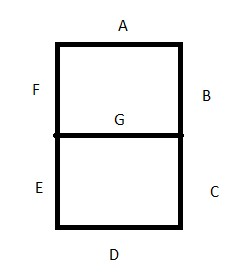
\includegraphics{convention.jpg}

    \end{figure}
\end{center}
Truth table:
\begin{center}
    \begin{tabular}{| c | c | c | c || c | c | c | c | c | c | c  |}
        \hline
        $W_3$ & $W_2$ & $W_1$ & $W_0$ & A & B & C & D & E & F & G \\
        \hline
        0     & 0     & 0     & 0     & 1 & 1 & 1 & 1 & 1 & 1 & 0 \\
        \hline
        0     & 0     & 0     & 1     & 0 & 1 & 1 & 0 & 0 & 0 & 0 \\
        \hline
        0     & 0     & 1     & 0     & 1 & 1 & 0 & 1 & 1 & 0 & 1 \\
        \hline
        0     & 0     & 1     & 1     & 1 & 1 & 1 & 1 & 0 & 0 & 1 \\
        \hline
        0     & 1     & 0     & 0     & 0 & 1 & 1 & 0 & 0 & 1 & 1 \\
        \hline
        0     & 1     & 0     & 1     & 1 & 0 & 1 & 1 & 0 & 1 & 1 \\
        \hline
        0     & 1     & 1     & 0     & 1 & 0 & 1 & 1 & 1 & 1 & 1 \\
        \hline
        0     & 1     & 1     & 1     & 1 & 1 & 1 & 0 & 0 & 0 & 0 \\
        \hline
        1     & 0     & 0     & 0     & 1 & 1 & 1 & 1 & 1 & 1 & 1 \\
        \hline
        1     & 0     & 0     & 1     & 1 & 1 & 1 & 1 & 0 & 1 & 1 \\
        \hline
    \end{tabular}
\end{center}
\newpage
The expressions realised from the above truth table:

\begin{align*}
    A & =W_3+W_1+W_2W_0+\bar{W_2}\bar{W_0}                                \\
    B & =\bar{W_2}+\bar{W_1}\bar{W_0}+W_1W_0                              \\
    C & =\bar{W_1}+W_0+W_2                                                \\
    D & =W_3+\bar{W_2}\bar{W_0}+\bar{W_2}W_1+W_1\bar{W_0}+W_2\bar{W_1}W_0 \\
    E & =\bar{W_2}\bar{W_0}+W_1\bar{W_0}                                  \\
    F & =W_3+W_2\bar{W_1}+\bar{W_1}\bar{W_0}+W_1\bar{W_0}                 \\
    G & =W_3+W_2\bar{W_0}+\bar{W_2}W_1+W_2\bar{W_1}                       \\
\end{align*}
\end{document}
